% Chapter 9: Prophet and TBATS
% Harvard-quality academic presentation
% Bachelor program, Bucharest University of Economic Studies

\documentclass[9pt, aspectratio=169, t]{beamer}

% Ensure content fits on slides
\setbeamersize{text margin left=8mm, text margin right=8mm}

%=============================================================================
% THEME AND STYLE CONFIGURATION
%=============================================================================
\usetheme{default}
% Using default theme for clean header/footer control

% Color Palette (matching Redispatch PDF)
\definecolor{MainBlue}{RGB}{26, 58, 110}
\definecolor{AccentBlue}{RGB}{26, 58, 110}
\definecolor{IDAred}{RGB}{205, 0, 0}
\definecolor{DarkGray}{RGB}{51, 51, 51}
\definecolor{MediumGray}{RGB}{128, 128, 128}
\definecolor{LightGray}{RGB}{248, 248, 248}
\definecolor{VeryLightGray}{RGB}{235, 235, 235}
\definecolor{KeynoteGray}{RGB}{218, 218, 218}
\definecolor{SectionGray}{RGB}{120, 120, 120}
\definecolor{FooterGray}{RGB}{100, 100, 100}
\definecolor{Crimson}{RGB}{220, 53, 69}
\definecolor{Forest}{RGB}{46, 125, 50}
\definecolor{Amber}{RGB}{181, 133, 63}
\definecolor{Orange}{RGB}{230, 126, 34}
\definecolor{Purple}{RGB}{142, 68, 173}

% Gradient background (exact Keynote 315° gradient: white to RGB 218,218,218)
\setbeamertemplate{background}{%
    \begin{tikzpicture}[remember picture, overlay]
        \shade[shading=axis, shading angle=315,
        top color=white, bottom color=KeynoteGray]
        (current page.south west) rectangle (current page.north east);
    \end{tikzpicture}%
}
% Fallback solid color for compatibility
\setbeamercolor{background canvas}{bg=}

\setbeamercolor{palette primary}{bg=MainBlue, fg=white}
\setbeamercolor{palette secondary}{bg=MainBlue!85, fg=white}
\setbeamercolor{palette tertiary}{bg=MainBlue!70, fg=white}
\setbeamercolor{structure}{fg=MainBlue}
\setbeamercolor{title}{fg=IDAred}
\setbeamercolor{frametitle}{fg=IDAred, bg=}
\setbeamercolor{block title}{bg=MainBlue, fg=white}
\setbeamercolor{block body}{bg=VeryLightGray, fg=DarkGray}
\setbeamercolor{block title alerted}{bg=Crimson, fg=white}
\setbeamercolor{block body alerted}{bg=Crimson!8, fg=DarkGray}
\setbeamercolor{block title example}{bg=Forest, fg=white}
\setbeamercolor{block body example}{bg=Forest!8, fg=DarkGray}
\setbeamercolor{item}{fg=MainBlue}

% Footer colors (override Madrid theme blue)
\setbeamercolor{author in head/foot}{fg=FooterGray, bg=}
\setbeamercolor{title in head/foot}{fg=FooterGray, bg=}
\setbeamercolor{date in head/foot}{fg=FooterGray, bg=}
\setbeamercolor{section in head/foot}{fg=FooterGray, bg=}
\setbeamercolor{subsection in head/foot}{fg=FooterGray, bg=}

% Bullet styles (apply everywhere including blocks)
\setbeamertemplate{itemize item}{\color{MainBlue}$\boxdot$}
\setbeamertemplate{itemize subitem}{\color{MainBlue}$\blacktriangleright$}
\setbeamertemplate{itemize subsubitem}{\color{MainBlue}\tiny$\bullet$}
\setbeamertemplate{itemize/enumerate body begin}{\normalsize}
\setbeamertemplate{itemize/enumerate subbody begin}{\normalsize}

% Item spacing - compact style
\setlength{\leftmargini}{10pt}       % Level 1: minimal indent
\setlength{\leftmarginii}{10pt}      % Level 2: minimal additional indent
% Compact list spacing (zero extra space before/after lists in blocks)
\makeatletter
\def\@listi{\leftmargin\leftmargini \topsep 0pt \parsep 0pt \itemsep 0pt}
\def\@listii{\leftmargin\leftmarginii \topsep 0pt \parsep 0pt \itemsep 0pt}
\makeatother

\setbeamertemplate{navigation symbols}{}

%=============================================================================
% CUSTOM HEADLINE
%=============================================================================
\setbeamertemplate{headline}{%
    \vskip10pt%
    \hbox to \paperwidth{%
        \hskip0.5cm%
        {\small\color{FooterGray}\renewcommand{\hyperlink}[2]{##2}\insertsectionhead}%
        \hfill%
        \textcolor{FooterGray}{\small\insertframenumber}%
        \hskip0.5cm%
    }%
    \vskip4pt%
    {\color{FooterGray}\hrule height 0.4pt}%
}

%=============================================================================
% CUSTOM FOOTER
%=============================================================================
\usepackage{fontawesome5}

\setbeamertemplate{footline}{%
    {\color{FooterGray}\hrule height 0.4pt}%
    \vskip4pt%
    \hbox to \paperwidth{%
        \hskip0.5cm%
        \textcolor{FooterGray}{\small Time Series Analysis and Forecasting}%
        \hfill%
        \raisebox{-0.1em}{%
            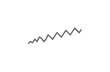
\begin{tikzpicture}[x=0.08em, y=0.08em, line width=0.4pt]
                \draw[FooterGray] (0,3) -- (1,4) -- (2,3.5) -- (3,5) -- (4,4) -- (5,6) -- (6,5.5) -- (7,4) -- (8,5) -- (9,7) -- (10,6) -- (11,5) -- (12,6.5) -- (13,8) -- (14,7) -- (15,6) -- (16,7.5) -- (17,9) -- (18,8) -- (19,7) -- (20,8.5) -- (21,10) -- (22,9) -- (23,8) -- (24,9.5);
            \end{tikzpicture}%
        }%
        \hskip0.5cm%
    }%
    \vskip6pt%
}

%=============================================================================
% PACKAGES
%=============================================================================
\usepackage[utf8]{inputenc}
\usepackage[T1]{fontenc}
\usepackage{amsmath, amssymb, amsthm}
\usepackage{mathtools}
\usepackage{bm}
\usepackage{tikz}
\usetikzlibrary{arrows.meta, positioning, shapes, calc, decorations.pathreplacing, shadings}
\usepackage{booktabs}
\usepackage{multirow}
\usepackage{array}
\usepackage{graphicx}
\usepackage{hyperref}
\usepackage{colortbl}
\hypersetup{colorlinks=true, linkcolor=MainBlue, urlcolor=MainBlue}
\graphicspath{{../../logos/}{../../charts/}{../../photos/}}
\hfuzz=2pt  % Suppress tiny overfull warnings (<2pt)
\vfuzz=2pt  % Suppress tiny vertical overfull warnings (<2pt)

%=============================================================================
% QUANTLET COMMAND
%=============================================================================
\newcommand{\quantlet}[2]{%
    \hfill\href{#2}{%
        \raisebox{-0.15em}{\includegraphics[height=0.7em]{ql_logo.png}}%
        \textcolor{MainBlue}{\tiny\ #1}%
    }%
}

%=============================================================================
% CUSTOM TITLE PAGE
%=============================================================================
\defbeamertemplate*{title page}{hybrid}[1][]
{
    \vspace{0.2cm}
    % Logos row - top header (with clickable links)
    \begin{center}
        \href{https://www.ase.ro}{\includegraphics[height=1.0cm]{ase_logo.png}}\hspace{0.3cm}%
        \href{https://theida.net}{\includegraphics[height=1.0cm]{ida_logo.png}}\hspace{0.3cm}%
        \href{https://blockchain-research-center.com}{\includegraphics[height=1.0cm]{brc_logo.png}}\hspace{0.3cm}%
        \href{https://www.ai4efin.ase.ro}{\includegraphics[height=1.0cm]{ai4efin_logo.png}}\hspace{0.3cm}%
        \href{https://ipe.ro/new}{\includegraphics[height=1.0cm]{acad_logo.png}}\hspace{0.3cm}%
        \href{https://www.digital-finance-msca.com}{\includegraphics[height=1.0cm]{msca_logo.png}}%
    \end{center}

    \vspace{0.6cm}

    % Main title with Q logos on sides (with clickable links)
    \begin{center}
        \begin{minipage}{0.1\textwidth}
            \centering
            \href{https://quantlet.com}{\includegraphics[height=1.1cm]{ql_logo.png}}
        \end{minipage}%
        \begin{minipage}{0.78\textwidth}
            \centering
            {\LARGE\bfseries\usebeamercolor[fg]{title}\inserttitle}

            \vspace{0.3cm}

            {\usebeamerfont{subtitle}\usebeamercolor[fg]{title}\insertsubtitle}
        \end{minipage}%
        \begin{minipage}{0.1\textwidth}
            \centering
            \href{https://quantinar.com}{\includegraphics[height=1.1cm]{qr_logo.png}}
        \end{minipage}
    \end{center}

    \vspace{0.6cm}

    % Authors (left aligned)
    \hspace{0.5cm}{\usebeamerfont{author}\insertauthor}

    \vspace{0.3cm}

    % Institute/Affiliations (left aligned)
    \hspace{0.5cm}\begin{minipage}[t]{0.9\textwidth}
        \raggedright\small\insertinstitute
    \end{minipage}
}

%=============================================================================
% THEOREM ENVIRONMENTS
%=============================================================================
\theoremstyle{definition}
\setbeamertemplate{theorems}[numbered]
\newtheorem{defn}{Definition}
\newtheorem{thm}{Theorem}
\newtheorem{prop}{Proposition}
\newtheorem{rmk}{Remark}

%=============================================================================
% CUSTOM COMMANDS
%=============================================================================
\newcommand{\E}{\mathbb{E}}
\newcommand{\Var}{\text{Var}}
\newcommand{\Cov}{\text{Cov}}
\newcommand{\Corr}{\text{Corr}}
\newcommand{\R}{\mathbb{R}}
\newcommand{\N}{\mathbb{N}}
\newcommand{\Z}{\mathbb{Z}}
\newcommand{\B}{\mathbf{B}}
\newcommand{\imark}{\textcolor{MainBlue}{\textbullet}}
\newcommand{\RMSE}{\text{RMSE}}
\newcommand{\MAE}{\text{MAE}}
\newcommand{\MAPE}{\text{MAPE}}

%=============================================================================
% TITLE INFORMATION
%=============================================================================
\title[Time Series Analysis]{Time Series Analysis and Forecasting}
\subtitle{Chapter 9: Prophet and TBATS}
\author[D.T. Pele]{Daniel Traian PELE}
\institute{Bucharest University of Economic Studies\\
IDA Institute Digital Assets\\
Blockchain Research Center\\
AI4EFin Artificial Intelligence for Energy Finance\\
Romanian Academy, Institute for Economic Forecasting\\
MSCA Digital Finance}
\date{}

%=============================================================================
% CENTRED MINIPAGE
%=============================================================================
\newenvironment{cminipage}[1]{%
    \par\noindent\hfill\begin{minipage}{#1}\ignorespaces
}{%
    \end{minipage}\hfill\null\par
}

\begin{document}

% Title page (no header/footer)
{
\setbeamertemplate{headline}{}
\setbeamertemplate{footline}{}
\begin{frame}
    \titlepage
\end{frame}
}

%=============================================================================
% LEARNING OBJECTIVES
%=============================================================================
\begin{frame}{Learning Objectives}
    \begin{cminipage}{0.95\textwidth}
\begin{block}{By the end of this chapter, you will be able to:}
\begin{itemize}\setlength{\itemsep}{0pt}
    \item Handle time series with multiple seasonal patterns
    \item Use Facebook Prophet for flexible forecasting with holidays
    \item Apply TBATS models for complex seasonality
    \item Compare and select between modern forecasting methods
\end{itemize}
\end{block}
    \end{cminipage}
\end{frame}

%=============================================================================
% TABLE OF CONTENTS
%=============================================================================
\begin{frame}{Outline}
    \vspace{-0.3cm}
    {\small
    \tableofcontents
    }
\end{frame}

%=============================================================================
% SECTION 1: MOTIVATION
%=============================================================================
\section{Multiple Seasonalities}

\begin{frame}{The Problem: Complex Seasonal Patterns}
    \begin{cminipage}{0.95\textwidth}
    \begin{block}{Real-World Examples}
        \begin{itemize}\setlength{\itemsep}{0pt}
            \item \textbf{Hourly electricity demand}: Daily + Weekly + Annual patterns
            \item \textbf{Website traffic}: Daily + Weekly + Holiday effects
            \item \textbf{Retail sales}: Weekly + Monthly + Annual + Holiday effects
            \item \textbf{Call center volume}:
                \begin{itemize}\setlength{\itemsep}{0pt}
                    \item Hourly + Daily + Weekly patterns
                \end{itemize}
            \end{itemize}
    \end{block}

    \vspace{0.3cm}

    \begin{alertblock}{SARIMA Limitation}
        Standard SARIMA$(p,d,q)(P,D,Q)_s$ handles only \textbf{one} seasonal period $s$.

        \vspace{0.2cm}
        For hourly data with daily AND weekly patterns, we need $s_1 = 24$ and $s_2 = 168$.
    \end{alertblock}
    \end{cminipage}
\end{frame}

\begin{frame}{Example: Hourly Data with Multiple Seasonalities}
    \begin{center}
        \includegraphics[width=0.95\textwidth, height=0.70\textheight, keepaspectratio]{ch9_multiple_seasonality.pdf}
    \end{center}
    \quantlet{TSA\_ch9\_multiple\_seasonality}{https://github.com/QuantLet/TSA/tree/main/TSA_ch9/TSA_ch9_multiple_seasonality}
\end{frame}

\begin{frame}{Solutions for Multiple Seasonalities}
    \vspace{-0.2cm}
    \begin{columns}[T]
        \column{0.5\textwidth}
        \begin{block}{Traditional Approaches}
            \begin{itemize}\setlength{\itemsep}{0pt}
                \item \textbf{Fourier terms}: Add sin/cos regressors
                \item \textbf{Dummy variables}: Many parameters
                \item \textbf{Nested models}: Complex specification
            \end{itemize}
        \end{block}

        \column{0.5\textwidth}
        \begin{exampleblock}{Modern Approaches}
            \begin{itemize}\setlength{\itemsep}{0pt}
                \item \textbf{TBATS}: Automatic, handles many periods
                \item \textbf{Prophet}: Flexible, interpretable
                \item \textbf{Neural methods}:
                \begin{itemize}\setlength{\itemsep}{0pt}
                    \item Deep learning
                \end{itemize}
            \end{itemize}
        \end{exampleblock}
    \end{columns}

    \vspace{0.5cm}

    \begin{center}
        \begin{tabular}{lcc}
            \toprule
            \textbf{Method} & \textbf{Max Seasonalities} & \textbf{Interpretable} \\
            \midrule
            SARIMA & 1 & Yes \\
            Fourier + ARIMA & Multiple & Moderate \\
            TBATS & Multiple & Moderate \\
            Prophet & Multiple & Yes \\
            \bottomrule
        \end{tabular}
    \end{center}
\end{frame}

\begin{frame}{Real Example: Electricity Demand}
    \begin{center}
        \includegraphics[width=0.95\textwidth, height=0.70\textheight, keepaspectratio]{ch9_electricity_demand.pdf}
    \end{center}
    \quantlet{TSA\_ch9\_electricity\_demand}{https://github.com/QuantLet/TSA/tree/main/TSA_ch9/TSA_ch9_electricity_demand}
\end{frame}

\begin{frame}{Real Example: Retail Sales with Holidays}
    \begin{center}
        \includegraphics[width=0.95\textwidth, height=0.70\textheight, keepaspectratio]{ch9_retail_sales.pdf}
    \end{center}
    \quantlet{TSA\_ch9\_retail\_sales}{https://github.com/QuantLet/TSA/tree/main/TSA_ch9/TSA_ch9_retail_sales}
\end{frame}

%=============================================================================
% SECTION 2: TBATS
%=============================================================================
\section{TBATS Model}

\begin{frame}{Researcher Spotlight: Rob J. Hyndman}
    \vspace{-0.3cm}
    \begin{columns}[T]
        \begin{column}{0.28\textwidth}
            \centering
            \includegraphics[width=0.95\textwidth, height=0.44\textheight, keepaspectratio]{photo_rob_hyndman.jpg}
            \\[0.15cm]
            {\footnotesize\textcolor{MediumGray}{*1967}}\\[0.05cm]
            \href{https://en.wikipedia.org/wiki/Rob_J._Hyndman}{\faWikipediaW\ \textcolor{MainBlue}{\small Wikipedia}}
        \end{column}
        \begin{column}{0.70\textwidth}
            {\footnotesize
            \begin{block}{Biography}
                \begin{itemize}\setlength{\itemsep}{0pt}
                    \item Australian statistician, Professor at Monash University
                    \item One of the most influential researchers in time series forecasting
                    \item Creator of the widely-used \texttt{forecast} package for R
                    \item Editor-in-Chief of the \textit{International Journal of Forecasting} (2005--2018)
                \end{itemize}
            \end{block}
            \begin{exampleblock}{Key Contributions}
                \begin{itemize}\setlength{\itemsep}{0pt}
                    \item \textbf{TBATS model} (2011) --- trigonometric Box-Cox ARMA with multiple seasonal periods
                    \item \textbf{ETS framework} --- exponential smoothing state space models with automatic selection
                    \item \textbf{forecast package} for R --- the standard toolkit for time series forecasting
                    \item \textbf{Hierarchical forecasting} and forecast reconciliation methods
                \end{itemize}
            \end{exampleblock}
            }
        \end{column}
    \end{columns}
\end{frame}

\begin{frame}{TBATS: What Does It Stand For?}
    \begin{cminipage}{0.95\textwidth}
    \begin{block}{TBATS Components}
        \begin{description}
            \item[T] \textbf{Trigonometric} seasonality using Fourier terms
            \item[B] \textbf{Box-Cox} transformation for variance stabilization
            \item[A] \textbf{ARMA} errors for remaining autocorrelation
            \item[T] \textbf{Trend} component (possibly damped)
            \item[S] \textbf{Seasonal} components (multiple allowed)
        \end{description}
    \end{block}

    \vspace{0.2cm}

    \begin{exampleblock}{Key Innovation: Trigonometric Seasonality}
        \[
        s_t^{(i)} = \sum_{j=1}^{k_i} \left[ s_j^{(i)} \cos\left(\frac{2\pi j t}{m_i}\right) + s_j^{*(i)} \sin\left(\frac{2\pi j t}{m_i}\right) \right]
        \]
        {\small $m_i$ = seasonal period, $k_i$ = number of harmonics}
    \end{exampleblock}
    \end{cminipage}
\end{frame}

\begin{frame}{Box-Cox Transformation}
    \begin{cminipage}{0.95\textwidth}
    \begin{defn}[Box-Cox Transformation]
        The Box-Cox transformation with parameter $\omega$ is defined as:
        \[
        y_t^{(\omega)} = \begin{cases}
            \dfrac{y_t^{\omega} - 1}{\omega} & \text{if } \omega \neq 0 \\[0.3cm]
            \ln(y_t) & \text{if } \omega = 0
        \end{cases}
        \]
    \end{defn}

    \vspace{0.2cm}

    \begin{exampleblock}{Purpose}
        \begin{itemize}\setlength{\itemsep}{0pt}
            \item \textbf{Variance stabilization}: Makes variance constant over time
            \item \textbf{Normalization}: Reduces skewness in the data
            \item Common values: $\omega = 0$ (log), $\omega = 0.5$ (square root), $\omega = 1$ (no transform)
        \end{itemize}
    \end{exampleblock}
    \end{cminipage}
\end{frame}

\begin{frame}{TBATS Model Structure}
    \begin{cminipage}{0.95\textwidth}
    \vspace{-0.3cm}
    {\small
    \begin{block}{State Space Representation}
        \begin{align}
            y_t^{(\omega)} &= \ell_{t-1} + \phi b_{t-1} + \sum_{i=1}^{T} s_{t-m_i}^{(i)} + d_t \\
            \ell_t &= \ell_{t-1} + \phi b_{t-1} + \alpha d_t, \quad b_t = \phi b_{t-1} + \beta d_t
        \end{align}
    \end{block}

    {\small
    \begin{columns}[T]
        \column{0.5\textwidth}
        \begin{itemize}\setlength{\itemsep}{0pt}
            \item $y_t^{(\omega)}$: Box-Cox transformed observation
            \item $\ell_t$: local level (smoothed mean)
            \item $b_t$: trend with damping $\phi \in (0,1)$
        \end{itemize}

        \column{0.5\textwidth}
        \begin{itemize}\setlength{\itemsep}{0pt}
            \item $s_t^{(i)}$: $i$-th seasonal component
            \item $d_t$: ARMA$(p,q)$ error process
            \item $\alpha, \beta$: smoothing parameters
        \end{itemize}
    \end{columns}
    }
    }
    \end{cminipage}
\end{frame}

\begin{frame}{TBATS: Trigonometric Seasonality State Evolution}
    \begin{cminipage}{0.95\textwidth}
    \begin{defn}[Trigonometric State-Space Recursion]
        For each seasonal component with period $m_i$ and $k_i$ harmonics, define states:
        \[
        \begin{pmatrix} s_{j,t}^{(i)} \\ s_{j,t}^{*(i)} \end{pmatrix} =
        \begin{pmatrix} \cos(\lambda_j) & \sin(\lambda_j) \\ -\sin(\lambda_j) & \cos(\lambda_j) \end{pmatrix}
        \begin{pmatrix} s_{j,t-1}^{(i)} \\ s_{j,t-1}^{*(i)} \end{pmatrix} +
        \begin{pmatrix} \gamma_1^{(i)} \\ \gamma_2^{(i)} \end{pmatrix} d_t
        \]
        where $\lambda_j = \frac{2\pi j}{m_i}$ is the $j$-th harmonic frequency.
    \end{defn}

    \vspace{0.2cm}

    \begin{block}{Interpretation}
        \begin{itemize}\setlength{\itemsep}{0pt}
            \item The rotation matrix preserves the periodic structure
            \item Total seasonal: $s_t^{(i)} = \sum_{j=1}^{k_i} s_{j,t}^{(i)}$
            \item Parameters: $2k_i$ states per seasonal period
        \end{itemize}
    \end{block}
    \end{cminipage}
\end{frame}

\begin{frame}{Fourier Approximation of Seasonality}
    \begin{center}
        \includegraphics[width=0.95\textwidth, height=0.70\textheight, keepaspectratio]{ch9_fourier_approximation.pdf}
    \end{center}
    \quantlet{TSA\_ch9\_fourier\_approximation}{https://github.com/QuantLet/TSA/tree/main/TSA_ch9/TSA_ch9_fourier_approximation}
\end{frame}

\begin{frame}{TBATS: Choosing the Number of Harmonics}
    \begin{block}{Why Fourier/Trigonometric Terms?}
        \begin{enumerate}\setlength{\itemsep}{0pt}
            \item \textbf{Parsimonious}: $2k$ parameters vs $m$ dummy variables
            \item \textbf{Smooth}: Captures smooth seasonal patterns naturally
            \item \textbf{Flexible}: Number of harmonics $k$ controls complexity
            \item \textbf{Non-integer periods}: Can handle $s = 365.25$ for daily data
        \end{enumerate}
    \end{block}

    \vspace{0.2cm}

    \begin{columns}[T]
        \column{0.5\textwidth}
        \begin{exampleblock}{Low $k$ (few harmonics)}
            \begin{itemize}\setlength{\itemsep}{0pt}
                \item Smooth pattern
                \item Fewer parameters
                \item May miss sharp peaks
            \end{itemize}
        \end{exampleblock}

        \column{0.5\textwidth}
        \begin{alertblock}{High $k$ (many harmonics)}
            \begin{itemize}\setlength{\itemsep}{0pt}
                \item Can capture any pattern
                \item More parameters ($2k$ total)
                \item Maximum useful: $k \leq \lfloor m/2 \rfloor$
            \end{itemize}
        \end{alertblock}
    \end{columns}
\end{frame}

\begin{frame}{TBATS: Key Features}
    \begin{cminipage}{0.95\textwidth}
    \vspace{-0.2cm}
    {\small
    \begin{block}{Automatic Model Selection}
        TBATS automatically determines:
        \begin{itemize}\setlength{\itemsep}{0pt}
            \item Box-Cox parameter $\omega$ for variance stabilization
            \item Number of harmonics $k_i$ for each seasonal period
            \item ARMA orders $(p,q)$ for residual autocorrelation
            \item Damped vs non-damped trend specification
        \end{itemize}
    \end{block}

    \vspace{0.3cm}

    \begin{exampleblock}{BATS vs TBATS}
        \begin{itemize}\setlength{\itemsep}{0pt}
            \item \textbf{BATS}: Traditional seasonal states (dummy variables)
            \item \textbf{TBATS}: Trigonometric (Fourier) seasonal representation
            \item TBATS more parsimonious for long seasonal periods
        \end{itemize}
    \end{exampleblock}
    }
    \end{cminipage}
\end{frame}

\begin{frame}{TBATS Decomposition Example}
    \begin{center}
        \includegraphics[width=0.95\textwidth, height=0.70\textheight, keepaspectratio]{ch9_tbats_decomposition.pdf}
    \end{center}
    \quantlet{TSA\_ch9\_tbats\_decomposition}{https://github.com/QuantLet/TSA/tree/main/TSA_ch9/TSA_ch9_tbats_decomposition}
\end{frame}

\begin{frame}{TBATS: Advantages and Limitations}
    \begin{cminipage}{0.95\textwidth}
    \small
    \begin{columns}[T]
        \column{0.5\textwidth}
        \begin{exampleblock}{Advantages}
            \begin{itemize}\setlength{\itemsep}{0pt}
                \item Handles \textbf{multiple} seasonal periods
                \item \textbf{Automatic} model selection
                \item Handles \textbf{non-integer} periods (365.25)
                \item \textbf{Box-Cox} for heteroskedasticity
                \item Good for \textbf{high-frequency} data
            \end{itemize}
        \end{exampleblock}

        \column{0.5\textwidth}
        \begin{alertblock}{Limitations}
            \begin{itemize}\setlength{\itemsep}{0pt}
                \item \textbf{Computationally intensive}
                \item No \textbf{external regressors}
                \item Less \textbf{interpretable} than Prophet
                \item Can be \textbf{slow} for very long series
                \item Requires \textbf{sufficient data} per season
            \end{itemize}
        \end{alertblock}
    \end{columns}
    \end{cminipage}
\end{frame}

%=============================================================================
% SECTION 3: PROPHET
%=============================================================================
\section{Facebook Prophet}

\begin{frame}{Prophet: Overview}
    \begin{cminipage}{0.95\textwidth}
    \begin{block}{What is Prophet?}
        Forecasting procedure developed by Facebook (Meta) in 2017 for \textbf{business time series}:
        \begin{itemize}\setlength{\itemsep}{0pt}
            \item Strong seasonal effects (daily, weekly, yearly)
            \item Holiday effects and trend changes (changepoints)
            \item Handles missing data and outliers
        \end{itemize}
    \end{block}

    \vspace{0.2cm}

    \begin{exampleblock}{Key Philosophy: ``Analyst-in-the-loop''}
        Designed for analysts with domain knowledge but without time series expertise.
    \end{exampleblock}
    \end{cminipage}
\end{frame}

\begin{frame}{Prophet Model Structure}
    \begin{block}{Decomposition Approach}
        Prophet uses an \textbf{additive decomposition}:
        \[
        y(t) = g(t) + s(t) + h(t) + \varepsilon_t
        \]
    \end{block}

    \vspace{0.3cm}

    \begin{columns}[T]
        \column{0.33\textwidth}
        \begin{block}{$g(t)$: Trend}
            \begin{itemize}\setlength{\itemsep}{0pt}
                \item Linear or logistic
                \item Automatic changepoints
                \item Growth saturation
            \end{itemize}
        \end{block}

        \column{0.33\textwidth}
        \begin{block}{$s(t)$: Seasonality}
            \begin{itemize}\setlength{\itemsep}{0pt}
                \item Fourier series
                \item Multiple periods
                \item Custom seasonality
            \end{itemize}
        \end{block}

        \column{0.33\textwidth}
        \begin{block}{$h(t)$: Holidays}
            \begin{itemize}\setlength{\itemsep}{0pt}
                \item Country holidays
                \item Custom events
                \item Window effects
            \end{itemize}
        \end{block}
    \end{columns}
\end{frame}

\begin{frame}{Prophet: Seasonality Component}
    \vspace{-0.3cm}
    {\scriptsize
    {\small
        \begin{block}{Fourier Series Representation}
            \vspace{-0.2cm}
            \[
            s(t) = \sum_{n=1}^{N} \left[ a_n \cos\left(\frac{2\pi n t}{P}\right) + b_n \sin\left(\frac{2\pi n t}{P}\right) \right]
            \]
            \vspace{-0.2cm}
        \end{block}

        \begin{exampleblock}{Default Settings}
            \begin{center}
            \small
            \begin{tabular}{lcc}
                \toprule
                \textbf{Seasonality} & \textbf{Period} & \textbf{Fourier Order} \\
                \midrule
                Yearly & 365.25 days & 10 \\
                Weekly & 7 days & 3 \\
                Daily & 1 day & 4 \\
                \bottomrule
            \end{tabular}
            \end{center}
            \vspace{-0.1cm}
            {\small Higher $N$ = more flexibility but risk of overfitting}
        \end{exampleblock}
        }
    }
    \vspace{-0.1cm}
    \begin{center}
        \includegraphics[width=0.95\textwidth, height=0.18\textheight, keepaspectratio]{ch9_prophet_components.pdf}
    \end{center}
    \quantlet{TSA\_ch9\_prophet\_components}{https://github.com/QuantLet/TSA/tree/main/TSA_ch9/TSA_ch9_prophet_components}
\end{frame}

\begin{frame}{Prophet: Trend Component}
    \begin{cminipage}{0.95\textwidth}
    \vspace{-0.2cm}
    {\small
    \begin{columns}[T]
        \column{0.55\textwidth}
        \begin{block}{Linear Trend with Changepoints}
            \[
            g(t) = (k + \bm{a}(t)^T \bm{\delta}) \cdot t + (m + \bm{a}(t)^T \bm{\gamma})
            \]
            {\small
            \begin{itemize}\setlength{\itemsep}{0pt}
                \item $k$: base growth rate (slope)
                \item $\bm{\delta} = (\delta_1, \ldots, \delta_S)$: slope changes at $S$ changepoints
                \item $\bm{a}(t) \in \{0,1\}^S$: indicator if changepoint $s$ is active at time $t$
            \end{itemize}
            }
        \end{block}

        \column{0.45\textwidth}
        \begin{exampleblock}{Logistic Growth}
            For saturating trends:
            \[
            g(t) = \frac{C(t)}{1 + e^{-(k + \bm{a}(t)^T\bm{\delta})(t-m-\bm{a}(t)^T\bm{\gamma})}}
            \]
            {\small $C(t)$ = time-varying carrying capacity}
        \end{exampleblock}
    \end{columns}

    \vspace{0.2cm}

    \begin{alertblock}{Continuity Constraint}
        The offset $\gamma_j = -s_j \cdot \delta_j$ ensures $g(t)$ is continuous at each changepoint $s_j$.
    \end{alertblock}
    }
    \end{cminipage}
\end{frame}

\begin{frame}{Trend Changepoint Detection}
    \begin{center}
        \includegraphics[width=0.95\textwidth, height=0.70\textheight, keepaspectratio]{ch9_changepoint_detection.pdf}
    \end{center}
    \quantlet{TSA\_ch9\_changepoint\_detection}{https://github.com/QuantLet/TSA/tree/main/TSA_ch9/TSA_ch9_changepoint_detection}
\end{frame}

\begin{frame}{Prophet: Holiday Effects}
    \begin{cminipage}{0.95\textwidth}
    \vspace{-0.15cm}
    \begin{block}{Holiday Model}
        \[
        h(t) = Z(t) \cdot \bm{\kappa}
        \]
        where $Z(t)$ is an indicator matrix for holidays and $\bm{\kappa}$ are holiday effects.
    \end{block}

    \vspace{0.3cm}

    \begin{columns}[T]
        \column{0.5\textwidth}
        \begin{exampleblock}{Built-in Features}
            \begin{itemize}\setlength{\itemsep}{0pt}
                \item 60+ countries supported
                \item Custom holiday definitions
                \item Window effects (before/after)
            \end{itemize}
        \end{exampleblock}

        \column{0.5\textwidth}
        \begin{block}{Holiday Types}
            \begin{itemize}\setlength{\itemsep}{0pt}
                \item National holidays
                \item Religious observances
                \item Business events
            \end{itemize}
        \end{block}
    \end{columns}
    \end{cminipage}
\end{frame}

\begin{frame}{Prophet: Customization Options}
    \begin{cminipage}{0.95\textwidth}
    \begin{block}{Seasonality Customization}
        \begin{itemize}\setlength{\itemsep}{0pt}
            \item Add custom seasonal periods (monthly, quarterly)
            \item Control Fourier order for each seasonality
            \item Enable/disable default seasonalities
        \end{itemize}
    \end{block}

    \vspace{0.3cm}

    \begin{exampleblock}{External Regressors}
        Prophet supports adding external variables:
        \begin{itemize}\setlength{\itemsep}{0pt}
            \item Weather data, promotions, special events
            \item Binary or continuous regressors
            \item Automatic regularization
        \end{itemize}
    \end{exampleblock}
    \end{cminipage}
\end{frame}

\begin{frame}{Prophet: Uncertainty Quantification}
    \begin{block}{Bayesian Framework}
        Prophet uses a \textbf{Laplace prior} on changepoint magnitudes:
        \[
        \delta_j \sim \text{Laplace}(0, \tau), \quad \tau = \texttt{changepoint\_prior\_scale}
        \]
        Smaller $\tau$ = sparser, smaller changepoints (more regularization).
    \end{block}

    \vspace{0.2cm}

    \begin{columns}[T]
        \column{0.5\textwidth}
        \begin{block}{Sources of Uncertainty}
            \begin{enumerate}\setlength{\itemsep}{0pt}
                \item \textbf{Trend}: Future changepoints
                \item \textbf{Seasonality}: Coefficient variance
                \item \textbf{Observation}: Residual noise $\sigma^2$
            \end{enumerate}
        \end{block}

        \column{0.5\textwidth}
        \begin{exampleblock}{Prediction Intervals}
            \begin{itemize}\setlength{\itemsep}{0pt}
                \item MAP estimation for point forecasts
                \item Monte Carlo sampling for intervals
                \item Default: 80\% credible interval
            \end{itemize}
        \end{exampleblock}
    \end{columns}
\end{frame}

\begin{frame}{Prophet: Tuning Parameters}
    \begin{cminipage}{0.95\textwidth}
    \begin{block}{Key Parameters}
        \begin{center}
        \small
        \begin{tabular}{p{4cm}p{8cm}}
            \toprule
            \textbf{Parameter} & \textbf{Effect} \\
            \midrule
            \texttt{changepoint\_prior\_scale} & Trend flexibility (default: 0.05) \\
            \texttt{seasonality\_prior\_scale} & Seasonality flexibility (default: 10) \\
            \texttt{holidays\_prior\_scale} & Holiday effect size (default: 10) \\
            \texttt{seasonality\_mode} & 'additive' or 'multiplicative' \\
            \texttt{changepoint\_range} & Portion of history for changepoints \\
            \bottomrule
        \end{tabular}
        \end{center}
    \end{block}

    \vspace{0.3cm}

    \begin{exampleblock}{Practical Tips}
        \begin{itemize}\setlength{\itemsep}{0pt}
            \item \textbf{Overfitting trend?} Decrease \texttt{changepoint\_prior\_scale}
            \item \textbf{Underfitting seasonality?} Increase \texttt{seasonality\_prior\_scale}
            \item \textbf{Seasonal amplitude varies?} Use \texttt{seasonality\_mode='multiplicative'}
        \end{itemize}
    \end{exampleblock}
    \end{cminipage}
\end{frame}

\begin{frame}{Additive vs Multiplicative Seasonality}
    \begin{cminipage}{0.95\textwidth}
    \begin{center}
        \includegraphics[width=0.95\textwidth, height=0.70\textheight, keepaspectratio]{ch9_additive_vs_multiplicative.pdf}
    \end{center}
    \quantlet{TSA\_ch9\_additive\_vs\_multiplicative}{https://github.com/QuantLet/TSA/tree/main/TSA_ch9/TSA_ch9_additive_vs_multiplicative}
    \end{cminipage}
\end{frame}

\begin{frame}{Prophet: Advantages and Limitations}
    \begin{cminipage}{0.95\textwidth}
    \small
    \begin{columns}[T]
        \column{0.5\textwidth}
        \begin{exampleblock}{Advantages}
            \begin{itemize}\setlength{\itemsep}{0pt}
                \item \textbf{Easy to use}: Minimal tuning needed
                \item \textbf{Interpretable}: Clear decomposition
                \item \textbf{Handles missing data} well
                \item \textbf{Holiday effects} built-in
                \item \textbf{Multiple seasonalities}
                \item \textbf{External regressors} supported
                \item \textbf{Fast} fitting
            \end{itemize}
        \end{exampleblock}

        \column{0.5\textwidth}
        \begin{alertblock}{Limitations}
            \begin{itemize}\setlength{\itemsep}{0pt}
                \item \textbf{Not ARIMA-based}: No autocorrelation modeling
                \item \textbf{Daily data focus}: Less suited for very high frequency
                \item \textbf{Trend assumptions}: Linear/logistic may not fit
                \item \textbf{No built-in CV}: Must implement manually
                \item \textbf{Overfitting risk} with many seasonalities
            \end{itemize}
        \end{alertblock}
    \end{columns}
    \end{cminipage}
\end{frame}

%=============================================================================
% SECTION 4: COMPARISON
%=============================================================================
\section{Comparison and Guidelines}

\begin{frame}{TBATS vs Prophet: Head-to-Head}
    \begin{cminipage}{0.95\textwidth}
    \vspace{-0.2cm}
    \begin{center}
    \small
    \begin{tabular}{p{4cm}p{4.5cm}p{4.5cm}}
        \toprule
        \textbf{Feature} & \textbf{TBATS} & \textbf{Prophet} \\
        \midrule
        Multiple seasonalities & Yes (automatic) & Yes (manual or auto) \\
        Holiday effects & No & Yes (built-in) \\
        External regressors & No & Yes \\
        Trend changepoints & No (smooth) & Yes (automatic) \\
        Missing data & Interpolation needed & Handles natively \\
        Interpretability & Moderate & High \\
        Computation speed & Slow & Fast \\
        High-frequency data & Good & Moderate \\
        Non-integer periods & Yes (e.g., 365.25) & Yes \\
        Uncertainty intervals & Yes & Yes \\
        \bottomrule
    \end{tabular}
    \end{center}
    \end{cminipage}
\end{frame}

\begin{frame}{When to Use Each Model}
    \begin{columns}[T]
        \column{0.5\textwidth}
        \begin{block}{Use TBATS when:}
            \begin{itemize}
                \item High-frequency data
                \item Multiple seasonal periods
                \item No external regressors
                \item Automatic selection preferred
            \end{itemize}
        \end{block}

        \column{0.5\textwidth}
        \begin{block}{Use Prophet when:}
            \begin{itemize}
                \item Business forecasting
                \item Holiday effects important
                \item Trend has changepoints
                \item External regressors available
            \end{itemize}
        \end{block}
    \end{columns}

    \vspace{0.3cm}

    \begin{exampleblock}{General Guideline}
        \begin{center}
            \textbf{Prophet}: business applications with daily data\\
            \textbf{TBATS}: technical applications with high-frequency data
        \end{center}
    \end{exampleblock}
\end{frame}

\begin{frame}{Decision Flowchart}
    \begin{cminipage}{0.95\textwidth}
    \begin{center}
    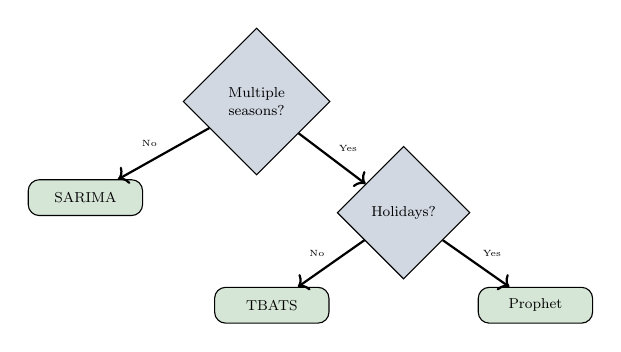
\begin{tikzpicture}[
        scale=0.65, transform shape,
        node distance=1cm,
        decision/.style={diamond, draw, fill=MainBlue!20, text width=2.2cm, text centered, inner sep=1pt, font=\footnotesize},
        block/.style={rectangle, draw, fill=Forest!20, text width=2cm, text centered, rounded corners, minimum height=0.7cm, font=\footnotesize},
        line/.style={draw, ->, thick}
    ]
        \node [decision] (q1) {Multiple seasons?};
        \node [block, below left=0.8cm and 1.5cm of q1] (sarima) {SARIMA};
        \node [decision, below right=0.8cm and 1.5cm of q1] (q2) {Holidays?};
        \node [block, below left=0.8cm and 0.8cm of q2] (tbats) {TBATS};
        \node [block, below right=0.8cm and 0.8cm of q2] (prophet) {Prophet};

        \path [line] (q1) -- node[above left, font=\tiny] {No} (sarima);
        \path [line] (q1) -- node[above right, font=\tiny] {Yes} (q2);
        \path [line] (q2) -- node[above left, font=\tiny] {No} (tbats);
        \path [line] (q2) -- node[above right, font=\tiny] {Yes} (prophet);
    \end{tikzpicture}
    \end{center}
    \end{cminipage}
\end{frame}

\begin{frame}{Prophet vs TBATS: Forecast Comparison}
    \begin{center}
        \includegraphics[width=0.95\textwidth, height=0.70\textheight, keepaspectratio]{ch9_prophet_vs_tbats.pdf}
    \end{center}
    \quantlet{TSA\_ch9\_prophet\_vs\_tbats}{https://github.com/QuantLet/TSA/tree/main/TSA_ch9/TSA_ch9_prophet_vs_tbats}
\end{frame}

\begin{frame}{Model Selection Guide}
    \vspace{-0.2cm}
    \begin{center}
        \includegraphics[width=0.95\textwidth, height=0.78\textheight, keepaspectratio]{ch9_model_selection_guide.pdf}
    \end{center}
    \quantlet{TSA\_ch9\_model\_selection\_guide}{https://github.com/QuantLet/TSA/tree/main/TSA_ch9/TSA_ch9_model_selection_guide}
\end{frame}

%=============================================================================
% SECTION 5: PRACTICAL EXAMPLE
%=============================================================================
\section{Case Study}

\begin{frame}{Evaluation Metrics}
    \vspace{-0.5cm}
    \begin{cminipage}{0.95\textwidth}
    \begin{defn}[Forecast Accuracy Metrics]
        Let $y_t$ denote actual values, $\hat{y}_t$ forecasts, and $n$ the forecast horizon:
        \begin{align*}
            \RMSE &= \sqrt{\frac{1}{n}\sum_{t=1}^{n}(y_t - \hat{y}_t)^2} \quad \text{(penalizes large errors)} \\
            \MAE &= \frac{1}{n}\sum_{t=1}^{n}|y_t - \hat{y}_t| \quad \text{(robust to outliers)} \\
            \MAPE &= \frac{100\%}{n}\sum_{t=1}^{n}\left|\frac{y_t - \hat{y}_t}{y_t}\right| \quad \text{(scale-free)}
        \end{align*}
    \end{defn}

    \begin{exampleblock}{Coverage}
        For prediction intervals $[\hat{y}_t^L, \hat{y}_t^U]$, coverage rate is the proportion of actual values falling within the interval. Target: match the nominal level (e.g., 80\%).
    \end{exampleblock}
    \end{cminipage}
\end{frame}

\begin{frame}{Case Study: Energy Demand Forecasting}
    \begin{cminipage}{0.95\textwidth}
    \begin{block}{Problem}
        Forecast hourly electricity demand with:
        \begin{itemize}\setlength{\itemsep}{0pt}
            \item \textbf{Daily pattern}: Peak at noon and evening
            \item \textbf{Weekly pattern}: Lower on weekends
            \item \textbf{Annual pattern}: Higher in summer (AC) and winter (heating)
            \item \textbf{Holiday effects}: Lower demand on holidays
        \end{itemize}
    \end{block}

    \vspace{0.3cm}

    \begin{exampleblock}{Approach}
        \begin{enumerate}\setlength{\itemsep}{0pt}
            \item Try TBATS with periods [24, 168, 8766]
            \item Try Prophet with daily, weekly, yearly seasonality + holidays
            \item Compare using cross-validation
        \end{enumerate}
    \end{exampleblock}
    \end{cminipage}
\end{frame}

\begin{frame}{Case Study: Results}
    \begin{cminipage}{0.95\textwidth}
    \vspace{-0.3cm}
    {\footnotesize
    \begin{exampleblock}{Model Comparison}
        \begin{center}
        \small
        \begin{tabular}{lccc}
            \toprule
            \textbf{Model} & \textbf{MAPE} & \textbf{RMSE} & \textbf{Coverage} \\
            \midrule
            SARIMA (daily only) & 8.5\% & 450 MW & 75\% \\
            TBATS & 4.2\% & 220 MW & 82\% \\
            Prophet & 4.8\% & 250 MW & 85\% \\
            Prophet + holidays & 3.9\% & 200 MW & 88\% \\
            \bottomrule
        \end{tabular}
        \end{center}
    \end{exampleblock}

    \begin{alertblock}{Key Finding}
        Multiple seasonality models significantly outperform single-seasonality SARIMA.
    \end{alertblock}
    }
    \end{cminipage}
\end{frame}

%=============================================================================
\section{AI Use Case}
%=============================================================================

\begin{frame}{AI Exercise: Critical Thinking}
    \begin{cminipage}{0.95\textwidth}
    \vspace{-3mm}
    \begin{block}{\footnotesize Prompt to test in ChatGPT / Claude / Copilot}
        {\footnotesize
        ``I have 3 years of hourly energy consumption data. Use Facebook Prophet to forecast the next week. Include holidays and special events. Give me complete Python code.''
        }
    \end{block}
    \vspace{-2mm}
    {\footnotesize
    \textbf{Exercise}:
    \begin{enumerate}\setlength{\itemsep}{0pt}
        \item Run the prompt in an LLM of your choice and critically analyze the response.
        \item Does Prophet automatically detect multiple seasonalities (daily, weekly)?
        \item How are holidays specified? Country-specific or custom events?
        \item Does it use cross-validation with cutoffs (performance\_metrics)?
        \item Would TBATS be more appropriate for this frequency? Why or why not?
    \end{enumerate}
    }
    \vspace{-2mm}
    \begin{alertblock}{}
        {\footnotesize \textbf{Warning}: AI-generated code may run without errors and look professional. \textit{That does not mean it is correct.}}
    \end{alertblock}
    \end{cminipage}
\end{frame}

%=============================================================================
% SECTION 6: QUIZ
%=============================================================================
\section{Quiz}

\begin{frame}{Question 1}
    \begin{cminipage}{0.95\textwidth}
    \begin{alertblock}{Question}
        \begin{itemize}\setlength{\itemsep}{0pt}
            \item Why can't standard SARIMA$(p,d,q)(P,D,Q)_s$ model hourly electricity data with both daily and weekly patterns?
        \end{itemize}
    \end{alertblock}

    \vspace{0.3cm}

    \begin{block}{Answer Choices}

        \textcolor{MainBlue}{\textbf{(A)}} SARIMA can only handle one seasonal period $s$ at a time\\[3pt]

        \textcolor{MainBlue}{\textbf{(B)}} SARIMA requires normally distributed errors for multiple seasonalities\\[3pt]

        \textcolor{MainBlue}{\textbf{(C)}} SARIMA can handle multiple seasonalities but requires more data\\[3pt]

        \textcolor{MainBlue}{\textbf{(D)}} SARIMA only works with monthly or quarterly data

    \end{block}
    \end{cminipage}
\end{frame}

\begin{frame}{Question 1: Answer}
    \begin{cminipage}{0.95\textwidth}
    \vspace{-0.2cm}
    \begin{center}
        \includegraphics[width=0.98\textwidth, height=0.58\textheight, keepaspectratio]{ch9_quiz1_multiple_seasonality.pdf}
    \end{center}
    \vspace{-3mm}
    {\small
    \begin{exampleblock}{Answer: (A)}
    \begin{itemize}\setlength{\itemsep}{0pt}
        \item SARIMA handles only \textbf{one} seasonal period $s$. You cannot set $s=24$ (daily) and $s=168$ (weekly) simultaneously in a single SARIMA model.
    \end{itemize}
    \end{exampleblock}
    }
    \hfill\quantlet{TSA\_ch9\_quiz1\_multiple\_seasonality}{https://github.com/QuantLet/TSA/tree/main/TSA_ch9/TSA_ch9_quiz1_multiple_seasonality}
    \end{cminipage}
\end{frame}

\begin{frame}{Question 2}
    \begin{cminipage}{0.95\textwidth}
    \begin{alertblock}{Question}
        \begin{itemize}\setlength{\itemsep}{0pt}
            \item What does each letter in TBATS represent?
        \end{itemize}
    \end{alertblock}

    \vspace{0.3cm}

    \begin{block}{Answer Choices}

        \textcolor{MainBlue}{\textbf{(A)}} Trend, Bayes, Autoregressive, Time, Stationarity\\[3pt]

        \textcolor{MainBlue}{\textbf{(B)}} Trigonometric seasonality, Box-Cox, ARMA errors, Trend, Seasonal components\\[3pt]

        \textcolor{MainBlue}{\textbf{(C)}} Taylor, Box-Cox, ARIMA, Transformation, Smoothing\\[3pt]

        \textcolor{MainBlue}{\textbf{(D)}} Trigonometric, Bayesian, ARMA, Trend, Spectral analysis

    \end{block}
    \end{cminipage}
\end{frame}

\begin{frame}{Question 2: Answer}
    \begin{cminipage}{0.95\textwidth}
    \vspace{-0.2cm}
    \begin{center}
        \includegraphics[width=0.98\textwidth, height=0.58\textheight, keepaspectratio]{ch9_quiz2_tbats_components.pdf}
    \end{center}
    \vspace{-3mm}
    {\small
    \begin{exampleblock}{Answer: (B)}
    \begin{itemize}\setlength{\itemsep}{0pt}
        \item \textbf{T}rigonometric seasonality, \textbf{B}ox-Cox transformation, \textbf{A}RMA errors, \textbf{T}rend, \textbf{S}easonal components.
    \end{itemize}
    \end{exampleblock}
    }
    \hfill\quantlet{TSA\_ch9\_quiz2\_tbats\_components}{https://github.com/QuantLet/TSA/tree/main/TSA_ch9/TSA_ch9_quiz2_tbats_components}
    \end{cminipage}
\end{frame}

\begin{frame}{Question 3}
    \begin{cminipage}{0.95\textwidth}
    \begin{alertblock}{Question}
        \begin{itemize}\setlength{\itemsep}{0pt}
            \item What happens when we increase the number of Fourier harmonics $K$?
        \end{itemize}
    \end{alertblock}

    \vspace{0.3cm}

    \begin{block}{Answer Choices}

        \textcolor{MainBlue}{\textbf{(A)}} The model becomes simpler and more robust\\[3pt]

        \textcolor{MainBlue}{\textbf{(B)}} The model captures more complex seasonal patterns but risks overfitting\\[3pt]

        \textcolor{MainBlue}{\textbf{(C)}} The forecast horizon increases proportionally\\[3pt]

        \textcolor{MainBlue}{\textbf{(D)}} The seasonal period $s$ changes automatically

    \end{block}
    \end{cminipage}
\end{frame}

\begin{frame}{Question 3: Answer}
    \begin{cminipage}{0.95\textwidth}
    \vspace{-0.2cm}
    \begin{center}
        \includegraphics[width=0.98\textwidth, height=0.58\textheight, keepaspectratio]{ch9_quiz3_fourier_harmonics.pdf}
    \end{center}
    \vspace{-3mm}
    {\small
    \begin{exampleblock}{Answer: (B)}
    \begin{itemize}\setlength{\itemsep}{0pt}
        \item Higher $K$ captures more complex seasonal patterns but increases the risk of overfitting. The maximum is $K \leq s/2$.
    \end{itemize}
    \end{exampleblock}
    }
    \hfill\quantlet{TSA\_ch9\_quiz3\_fourier\_harmonics}{https://github.com/QuantLet/TSA/tree/main/TSA_ch9/TSA_ch9_quiz3_fourier_harmonics}
    \end{cminipage}
\end{frame}

\begin{frame}{Question 4}
    \begin{cminipage}{0.95\textwidth}
    \begin{alertblock}{Question}
        \begin{itemize}\setlength{\itemsep}{0pt}
            \item What are the main components in Prophet's model $y(t) = g(t) + s(t) + h(t) + \varepsilon_t$?
        \end{itemize}
    \end{alertblock}

    \vspace{0.3cm}

    \begin{block}{Answer Choices}

        \textcolor{MainBlue}{\textbf{(A)}} $g(t)$ = GARCH volatility, $s(t)$ = stationarity test, $h(t)$ = heteroskedasticity\\[3pt]

        \textcolor{MainBlue}{\textbf{(B)}} $g(t)$ = growth (trend with changepoints), $s(t)$ = seasonality, $h(t)$ = holiday effects\\[3pt]

        \textcolor{MainBlue}{\textbf{(C)}} $g(t)$ = Gaussian noise, $s(t)$ = smoothing, $h(t)$ = harmonic terms\\[3pt]

        \textcolor{MainBlue}{\textbf{(D)}} $g(t)$ = gradient, $s(t)$ = spectral density, $h(t)$ = Hurst exponent

    \end{block}
    \end{cminipage}
\end{frame}

\begin{frame}{Question 4: Answer}
    \begin{cminipage}{0.95\textwidth}
    \vspace{-0.2cm}
    \begin{center}
        \includegraphics[width=0.98\textwidth, height=0.58\textheight, keepaspectratio]{ch9_quiz4_prophet_decomposition.pdf}
    \end{center}
    \vspace{-3mm}
    {\small
    \begin{exampleblock}{Answer: (B)}
    \begin{itemize}\setlength{\itemsep}{0pt}
        \item $g(t)$ = trend with changepoints, $s(t)$ = seasonality (Fourier terms), $h(t)$ = holiday effects, $\varepsilon_t$ = error term.
    \end{itemize}
    \end{exampleblock}
    }
    \hfill\quantlet{TSA\_ch9\_quiz4\_prophet\_decomposition}{https://github.com/QuantLet/TSA/tree/main/TSA_ch9/TSA_ch9_quiz4_prophet_decomposition}
    \end{cminipage}
\end{frame}

\begin{frame}{Question 5}
    \begin{cminipage}{0.95\textwidth}
    \begin{alertblock}{Question}
        \begin{itemize}\setlength{\itemsep}{0pt}
            \item What key features does Prophet have that TBATS lacks?
        \end{itemize}
    \end{alertblock}

    \vspace{0.3cm}

    \begin{block}{Answer Choices}

        \textcolor{MainBlue}{\textbf{(A)}} Trigonometric seasonality and Box-Cox transformation\\[3pt]

        \textcolor{MainBlue}{\textbf{(B)}} Automatic parameter selection and exponential smoothing\\[3pt]

        \textcolor{MainBlue}{\textbf{(C)}} Holiday effects, external regressors, trend changepoints, and native missing data handling\\[3pt]

        \textcolor{MainBlue}{\textbf{(D)}} State-space formulation and ARMA error modeling

    \end{block}
    \end{cminipage}
\end{frame}

\begin{frame}{Question 5: Answer}
    \begin{cminipage}{0.95\textwidth}
    \vspace{-0.2cm}
    \begin{center}
        \includegraphics[width=0.98\textwidth, height=0.58\textheight, keepaspectratio]{ch9_quiz5_prophet_vs_tbats.pdf}
    \end{center}
    \vspace{-3mm}
    {\small
    \begin{exampleblock}{Answer: (C)}
    \begin{itemize}\setlength{\itemsep}{0pt}
        \item Prophet offers holiday effects, external regressors, trend changepoints, and native missing data handling---features not available in TBATS.
    \end{itemize}
    \end{exampleblock}
    }
    \hfill\quantlet{TSA\_ch9\_quiz5\_prophet\_vs\_tbats}{https://github.com/QuantLet/TSA/tree/main/TSA_ch9/TSA_ch9_quiz5_prophet_vs_tbats}
    \end{cminipage}
\end{frame}

%=============================================================================
% SECTION 7: SUMMARY
%=============================================================================
\section{Summary}

\begin{frame}{Key Takeaways}
\begin{block}{What We Learned}
\begin{itemize}
    \item TBATS handles multiple seasonalities with Fourier terms and Box-Cox transformation
    \item Prophet provides interpretable decomposition with trend changepoints and holiday effects
    \item Both methods scale better than SARIMA for high-frequency and complex seasonal data
\end{itemize}
\end{block}

\begin{alertblock}{Important}
Choose Prophet for business forecasting with holidays and interpretability needs. Use TBATS for automatic modeling of high-frequency data. Always validate with time series cross-validation---never standard k-fold!
\end{alertblock}
\end{frame}

\begin{frame}{Questions?}
    \begin{center}
        \Large\textcolor{MainBlue}{Questions?}

        \vspace{1cm}

        \normalsize
        \textbf{Next Steps:}
        \begin{itemize}
            \item Practice with the Jupyter notebook
            \item Try Prophet on your own data
            \item Explore NeuralProphet for deep learning extension
        \end{itemize}
    \end{center}
\end{frame}

\begin{frame}{Bibliography I}
    \begin{block}{Prophet}
        {\small
        \begin{itemize}\setlength{\itemsep}{0pt}
            \item Taylor, S.J., \& Letham, B. (2018). Forecasting at Scale, \textit{The American Statistician}, 72(1), 37--45.
            \item Harvey, A.C. (1989). \textit{Forecasting, Structural Time Series Models and the Kalman Filter}, Cambridge University Press.
        \end{itemize}
        }
    \end{block}

    \begin{exampleblock}{TBATS and Exponential Smoothing}
        {\small
        \begin{itemize}\setlength{\itemsep}{0pt}
            \item De Livera, A.M., Hyndman, R.J., \& Snyder, R.D. (2011). Forecasting Time Series with Complex Seasonal Patterns Using Exponential Smoothing, \textit{JASA}, 106(496), 1513--1527.
            \item Hyndman, R.J., Koehler, A.B., Ord, J.K., \& Snyder, R.D. (2008). \textit{Forecasting with Exponential Smoothing: The State Space Approach}, Springer.
            \item Taylor, J.W. (2003). Short-term Electricity Demand Forecasting Using Double Seasonal Exponential Smoothing, \textit{Journal of the Operational Research Society}, 54(8), 799--805.
        \end{itemize}
        }
    \end{exampleblock}
\end{frame}

\begin{frame}{Bibliography II}
    \begin{block}{Forecasting Comparisons and Competitions}
        {\small
        \begin{itemize}\setlength{\itemsep}{0pt}
            \item Makridakis, S., Spiliotis, E., \& Assimakopoulos, V. (2020). The M4 Competition, \textit{International Journal of Forecasting}, 36(1), 54--74.
            \item Hyndman, R.J., \& Athanasopoulos, G. (2021). \textit{Forecasting: Principles and Practice}, 3rd ed., OTexts.
            \item Petropoulos, F., et al. (2022). Forecasting: Theory and Practice, \textit{International Journal of Forecasting}, 38(3), 845--1054.
        \end{itemize}
        }
    \end{block}

    \begin{exampleblock}{Online Resources and Code}
        {\small
        \begin{itemize}\setlength{\itemsep}{0pt}
            \item \textbf{Quantlet}: \url{https://quantlet.com} $\succ$ Code repository for statistics
            \item \textbf{Quantinar}: \url{https://quantinar.com} $\succ$ Learning platform for quantitative methods
            \item \textbf{GitHub TSA}: \url{https://github.com/QuantLet/TSA/tree/main/TSA_ch9} $\succ$ Python code for this chapter
        \end{itemize}
        }
    \end{exampleblock}
\end{frame}

\begin{frame}{}
    \centering
    \Huge\textcolor{MainBlue}{Thank You!}

    \vspace{1cm}

    \Large Questions?

    \vspace{0.8cm}

    \normalsize

    Course materials available at: \url{https://danpele.github.io/Time-Series-Analysis/}

    \vspace{0.2cm}

    \href{https://quantlet.com}{\raisebox{-0.15em}{\includegraphics[height=0.8em]{ql_logo.png}} Quantlet} \hspace{0.5cm}
    \href{https://quantinar.com}{\raisebox{-0.15em}{\includegraphics[height=0.8em]{qr_logo.png}} Quantinar}
\end{frame}

\end{document}
